\documentclass[11pt,a4paper]{article}

% --- Paquetes de configuración básica y tipografía ---
\usepackage[utf8]{inputenc}
\usepackage[spanish,es-tabla]{babel}
\usepackage[margin=2.5cm]{geometry}
\usepackage{amsmath,amsfonts,amssymb}
\usepackage{graphicx}
\usepackage{booktabs}
\usepackage{tabularx}
\usepackage{longtable}
\usepackage{array}
\usepackage{caption}
\usepackage{subcaption}
\usepackage{float}
\usepackage{xcolor}
\usepackage{listings}
\usepackage{fancyhdr}
\usepackage{microtype}
\usepackage{enumitem}
\usepackage[hidelinks,colorlinks=true,linkcolor=blue!70!black,citecolor=blue!70!black,urlcolor=blue!70!black]{hyperref}

% --- Configuración de encabezados y pies de página ---
\pagestyle{fancy}
\fancyhf{}
\rhead{\footnotesize CC209 -- Data Mining Tools | TP1}
\lhead{\footnotesize Estimación del Precio de Departamentos en Lima}
\cfoot{\thepage}

% --- Formato de listados de código ---
\definecolor{codegray}{rgb}{0.5,0.5,0.5}
\definecolor{backcolour}{rgb}{0.97,0.97,0.98}
\definecolor{codeblue}{rgb}{0.13,0.13,0.7}
\lstdefinestyle{mystyle}{
    backgroundcolor=\color{backcolour},
    commentstyle=\color{codegray},
    keywordstyle=\color{codeblue}\bfseries,
    numberstyle=\tiny\color{codegray},
    basicstyle=\ttfamily\footnotesize,
    breakatwhitespace=false,
    breaklines=true,
    captionpos=b,
    keepspaces=true,
    numbers=left,
    numbersep=5pt,
    showspaces=false,
    showstringspaces=false,
    showtabs=false,
    tabsize=2
}
\lstset{style=mystyle}

\begin{document}

% ==============================================================================
% PORTADA INSTITUCIONAL
% ==============================================================================
\begin{titlepage}
    \centering
    
\includegraphics[width=0.28\textwidth]{figures/logo-upc-png-transparente-1.png}\\[0.6cm]
    
    {\scshape\Large \textbf{UNIVERSIDAD PERUANA DE CIENCIAS APLICADAS}}\\[0.2cm]
    {\scshape\normalsize Carrera de Ciencias de la Computación}\\[1.3cm]
    
    {\Large \textbf{TRABAJO PARCIAL 1 (TP1)}}\\[0.4cm]
    {\LARGE \textbf{Estimación Supervisada del Valor Comercial de Oferta Inmobiliaria en Lima Metropolitana}}\\[0.4cm]
    
    \textbf{\large Curso:}\\[0.1cm]
    {\normalsize Data Mining Tools (CC209) -- Ciclo 2026-1}\\[0.5cm]
    
    \textbf{\large Docente:}\\[0.1cm]
    {\normalsize Carlos Fernando Montoya Cubas}\\[0.6cm]
    
    \textbf{\large Integrantes:}\\[0.2cm]
    {\normalsize Piero Marcos Contreras Albornoz}\\[0.12cm]
    {\normalsize Guido Yair Abel Jeri Saldaña}\\[0.12cm]
    {\normalsize José Guillermo Melgar Puertas}\\[0.12cm]
    {\normalsize Gabriel Alonzo Reyna Alvarado}\\[0.8cm]
    
    \vfill
    {\normalsize Lima, Perú}\\[0.1cm]
    {\normalsize Octubre de 2026}
\end{titlepage}

\clearpage

% ==============================================================================
% RESUMEN EJECUTIVO (ABSTRACT)
% ==============================================================================
\begin{abstract}
El mercado inmobiliario de Lima Metropolitana se caracteriza por una alta dispersión de precios, fuerte asimetría de información y el uso extendido de heurísticas simplistas basadas únicamente en el precio mediano por metro cuadrado distrital. El presente proyecto aborda la estimación del precio de oferta (\textit{asking price}) en dólares estadounidenses para departamentos residenciales en Lima mediante técnicas de Machine Learning supervisado. A partir de la base de microdatos del Banco Central de Reserva del Perú (BCRP), compuesta por 119,980 anuncios trimestrales (1998--2026), se diseñó un flujo de preparación riguroso que comprende deduplicación, corrección lógica de atributos, normalización de grafías distritales y eliminación estricta de fuentes de fuga de datos (\textit{data leakage}). Para capturar la estructura contemporánea de mercado y la incorporación de 26 distritos, se acotó el modelado al período 2022--2026 (40,368 observaciones), empleando una partición temporal fuera de muestra (\textit{out-of-time}): 2022--2023 para entrenamiento ($N = 15,158$) y 2024--2026 para evaluación ($N = 25,048$). La variable objetivo se transformó logarítmicamente para modelar errores proporcionales. Se estructuró un flujo reproducible con \texttt{ColumnTransformer} y se evaluaron dos baselines (Dummy y regla empírica distrital) junto con cuatro algoritmos: Ridge, ElasticNet, Random Forest y CatBoost Regressor. Los resultados demuestran que los métodos basados en gradiente superan ampliamente la referencia comercial: CatBoost redujo el error porcentual mediano (MedAPE) a un \textbf{11.3\%} (frente al \textbf{14.9\%} de la regla de mercado) y el RMSE de US\$ 38,350 a \textbf{US\$ 32,685}, logrando que el \textbf{45.3\%} de las estimaciones presente un error inferior al 10\%. Finalmente, se diagnostican residuales en segmentos de lujo y zonas periféricas, y se formula la hoja de ruta hacia el Trabajo Final (TF1).
\end{abstract}

\clearpage
\tableofcontents
\clearpage

% ==============================================================================
\section{Definición del Problema}
% ==============================================================================

\subsection{Contexto del Problema}
En Lima Metropolitana, la adquisición y venta de bienes inmuebles representa una de las decisiones financieras y de inversión de mayor envergadura para personas naturales y empresas. Históricamente, los departamentos residenciales se anuncian, cotizan y negocian predominantemente en dólares corrientes de los Estados Unidos (US\$). 

Sin embargo, el mercado inmobiliario limeño opera en un entorno de marcada asimetría de información. A diferencia de mercados bursátiles o de activos financieros estandarizados, los precios de oferta no están centralizados en un registro único con cotizaciones públicas en tiempo real. Adicionalmente, el valor del metro cuadrado ha experimentado profundas transformaciones longitudinales: entre 2007 y 2014, el precio mediano por metro cuadrado se triplicó en la capital (pasando de US\$ 558 a US\$ 1,592), experimentando una etapa de estabilización hasta 2022 y un posterior ciclo de aceleración contemporánea (alcanzando US\$ 1,804 hacia 2025). En este escenario, cualquier tasación que no contemple tanto la localización como la época y atributos intrínsecos del inmueble corre el riesgo de quedar rápidamente desfasada.

\subsection{Necesidad o Situación que se Desea Abordar}
En la práctica comercial actual, los compradores particulares, agentes inmobiliarios y tasadores independientes recurren con frecuencia a reglas heurísticas simplificadas. La regla de mercado más difundida consiste en calcular el precio de un departamento multiplicando el metraje total por la mediana del valor unitario del distrito de referencia:
\begin{equation}
    \widehat{\text{Precio}} = \text{Mediana}\left(\frac{\text{US\$}}{\text{m}^2}\right)_{\text{distrito}} \times \text{Superficie (m}^2\text{)}
    \label{eq:regla_mercado}
\end{equation}
Si bien esta fórmula es fácil de comunicar, adolece de limitaciones estructurales críticas:
\begin{itemize}[leftmargin=1.5cm]
    \item \textbf{Omisión de dotaciones físicas clave:} Asume implícitamente que dos departamentos del mismo metraje y distrito tienen igual valor, ignorando el número de dormitorios, baños y la presencia de cocheras (cuyo valor marginal varía fuertemente entre distritos).
    \item \textbf{Desprecio de la depreciación:} No penaliza el deterioro ni premia el estreno, asignando el mismo ratio unitario a un edificio de 40 años que a un proyecto recién entregado.
    \item \textbf{Rigidez temporal:} Asume estabilidad en la prima espacial distrital sin internalizar dinámicas de oferta y demanda por trimestre.
\end{itemize}
Existe, por ende, la necesidad de construir una herramienta predictiva analítica basada en datos que permita valorar de forma multivariada y objetiva las propiedades, sirviendo como guía de referencia confiable para fijar precios de lista razonables o detectar sobreprecios.

\subsection{Unidad de Análisis}
La unidad de análisis corresponde a un \textbf{anuncio individual de venta de un departamento en Lima Metropolitana publicado en un trimestre determinado}. Cada fila de la base de datos representa la oferta de una propiedad con sus atributos declarados en un momento específico del tiempo, y no una transacción de compraventa final cerrada.

\subsection{Pregunta Principal del Proyecto}
\begin{quote}
    \textit{¿Con qué nivel de precisión (medido en error porcentual y absoluto) es posible estimar el precio de oferta en dólares de un departamento residencial en Lima Metropolitana a partir de su superficie, número de dormitorios, baños, garajes, antigüedad y distrito, evaluando sobre anuncios publicados en los trimestres más recientes mediante un esquema temporal fuera de muestra (\textit{out-of-time})?}
\end{quote}

\subsection{Tipo de Problema de Data Science}
Se trata de un problema de \textbf{regresión supervisada sobre datos tabulares}. La variable de respuesta es cuantitativa continua ($\text{precio\_usd} \in \mathbb{R}^+$). La modelación incorpora restricciones temporales estrictas: el entrenamiento se ejecuta sobre trimestres pasados y la evaluación se realiza sobre trimestres futuros, emulando con fidelidad las condiciones operativas de un sistema de tasación en producción.

\subsection{Utilidad Esperada de la Solución}
La solución proveerá un estimador algorítmico capaz de:
\begin{enumerate}[leftmargin=1.5cm]
    \item \textbf{Compradores:} Proveer un baremo cuantitativo objetivo para discernir si un inmueble anunciado se encuentra subvaluado (oportunidad comercial) o sobrevaluado frente a pares comparables.
    \item \textbf{Vendedores particulares y desarrolladores:} Determinar precios de lista competitivos que aceleren el tiempo de absorción en el mercado sin incurrir en castigos de precio innecesarios.
    \item \textbf{Entidades bancarias y corredores:} Detectar valores atípicos o anomalías de digitación en plataformas de corretaje inmobiliario.
\end{enumerate}

\subsection{Criterios de Utilidad del Resultado}
Para considerar que la solución desarrollada aporta un valor sustantivo frente a la práctica estándar del sector, se establecen los siguientes criterios cuantitativos de éxito:
\begin{enumerate}[leftmargin=1.5cm]
    \item \textbf{Superación del Baseline de Dominio:} El modelo debe batir de manera estadísticamente consistente la regla de mercado (\textit{mediana distrital US\$/m$^2$ $\times$ metraje}), no únicamente a baselines triviales como la media o mediana global.
    \item \textbf{Error Porcentual Mediano (MedAPE):} Reducir el error porcentual mediano general en el conjunto de prueba a un umbral no mayor al \textbf{12\%} (aspirando a niveles cercanos al 10\%).
    \item \textbf{Cobertura en Margen Comercial:} Lograr que al menos el \textbf{40\%} de las propiedades evaluadas presenten un error relativo de predicción igual o menor al \textbf{10\%}.
    \item \textbf{Consistencia Espacial:} Ningún distrito que posea una masa muestral representativa ($N > 200$ en prueba) deberá exhibir un error mediano superior al \textbf{20\%}.
\end{enumerate}

\noindent \textbf{Delimitación del alcance:} El modelo no pretende estimar el precio final transado ante notaría ni explicar causalidad econométrica (por ejemplo, el impacto causal aislado de una cochera sobre la plusvalía), sino capturar patrones predictivos de oferta.

% ==============================================================================
\section{Dataset y Procedencia}
% ==============================================================================

\subsection{Fuente y Procedencia}
La información proviene de la base desagregada de precios de venta de departamentos recopilada por el \textbf{Banco Central de Reserva del Perú (BCRP)}. El BCRP consolida estos microdatos para la elaboración de sus indicadores trimestrales de precios de activos y política monetaria:
\begin{itemize}[leftmargin=1.5cm]
    \item \textbf{Período 1998--2007:} Los registros se extrajeron sistemáticamente de avisos clasificados en diarios de circulación nacional (principalmente la sección inmobiliaria de \textit{El Comercio}).
    \item \textbf{Período 2008--2026:} La recolección migró a plataformas digitales especializadas, concentrándose en el portal líder del mercado peruano (\textit{Urbania}).
\end{itemize}
Los fundamentos metodológicos institucionales se encuentran documentados en el \textit{Documento de Trabajo BCRP N° 006-2018} y en la \textit{Nota de Estudios BCRP N° 65-2025}.

\subsection{Observaciones y Variables Brutas}
La base de datos original sin procesar presenta las características consolidadas en el Cuadro \ref{tab:ficha_tecnica}.

\begin{table}[H]
\centering
\small
\caption{Ficha técnica del dataset original del BCRP.}
\label{tab:ficha_tecnica}
\begin{tabularx}{0.85\textwidth}{lX}
\toprule
\textbf{Parámetro} & \textbf{Valor / Descripción} \\
\midrule
Fuente institucional & Banco Central de Reserva del Perú (BCRP) -- BCRPData \\
Observaciones brutas & 119,980 anuncios \\
Variables originales & 16 columnas \\
Rango temporal & 1998-Trimestre 1 a 2026-Trimestre 1 (113 trimestres, 29 años) \\
Distritos registrados (brutos) & 44 variantes de texto (26 distritos reales tras normalizar) \\
Filas duplicadas exactas & 2,730 observaciones \\
Variable objetivo de modelado & \texttt{precio\_usd} (Precio de oferta en dólares corrientes) \\
Régimen de almacenamiento & Archivo Parquet comprimido (\texttt{precios\_venta\_bcrp\_2026\_1.parquet}, 1.9 MB) \\
\bottomrule
\end{tabularx}
\end{table}

\subsection{Cobertura Geográfica y Expansión Longitudinal}
Uno de los hallazgos cruciales respecto a la procedencia radica en la cobertura territorial asimétrica por épocas, expuesta en el Cuadro \ref{tab:cobertura_distritos}.

\begin{table}[H]
\centering
\small
\caption{Evolución del número de anuncios recopilados por distrito según época.}
\label{tab:cobertura_distritos}
\begin{tabularx}{\textwidth}{lccccX}
\toprule
\textbf{Distrito} & \textbf{1998--2007} & \textbf{2008--2013} & \textbf{2014--2021} & \textbf{2022--2026} & \textbf{Estado de Cobertura} \\
\midrule
Santiago de Surco & 4,870 & 3,202 & 4,380 & 5,922 & Histórico (Lima Top) \\
Miraflores & 4,069 & 3,057 & 4,384 & 5,997 & Histórico (Lima Top) \\
San Borja & 3,128 & 1,812 & 2,944 & 2,565 & Histórico (Lima Top) \\
La Molina & 2,901 & 1,468 & 2,554 & 1,570 & Histórico (Lima Top) \\
San Isidro & 2,605 & 1,760 & 3,210 & 2,201 & Histórico (Lima Top) \\
San Miguel & 37 & 1,931 & 3,042 & 3,280 & Expandido desde 2008 \\
Magdalena del Mar & 30 & 1,649 & 2,481 & 2,342 & Expandido desde 2008 \\
Jesús María & 28 & 1,347 & 2,059 & 2,063 & Expandido desde 2008 \\
Pueblo Libre & 25 & 1,353 & 2,069 & 1,867 & Expandido desde 2008 \\
Lince & 19 & 1,013 & 1,683 & 1,639 & Expandido desde 2008 \\
Barranco & 6 & 628 & 1,320 & 1,597 & Expandido desde 2008 \\
Surquillo & 0 & 211 & 1,979 & 2,499 & Expandido desde 2008 \\
Ate Vitarte & 0 & 0 & 0 & 1,068 & Reciente (2022+) \\
Comas & 0 & 0 & 0 & 562 & Reciente (2022+) \\
La Victoria & 0 & 0 & 0 & 717 & Reciente (2022+) \\
\midrule
\textbf{Distritos activos} & \textbf{15 (sesgo a 5)} & \textbf{19} & \textbf{19} & \textbf{26} & \textbf{Cobertura metropolitana plena} \\
\bottomrule
\end{tabularx}
\end{table}

\noindent Los datos demuestran que durante la primera década (1998--2007), más del 95\% del volumen muestral pertenecía exclusivamente a 5 distritos de ingresos altos (\textit{Lima Top}: Surco, Miraflores, San Borja, La Molina y San Isidro). Recién a partir del año 2022 el BCRP incorporó sistemáticamente distritos populosos de Lima Norte y Este (Ate, Comas, La Victoria).

\subsection{Diccionario de Variables}
El Cuadro \ref{tab:diccionario} detalla las 16 variables del dataset original, su tipo de dato, presencia de nulos y el rol asignado en el proyecto.

\begin{table}[H]
\centering
\scriptsize
\caption{Diccionario de variables del dataset original del BCRP.}
\label{tab:diccionario}
\begin{tabularx}{\textwidth}{lp{3.5cm}cclX}
\toprule
\textbf{Variable} & \textbf{Descripción} & \textbf{Tipo} & \textbf{Nulos} & \textbf{Rango} & \textbf{Rol en el Proyecto} \\
\midrule
\texttt{periodo} & Código de trimestre (ej. \textit{'1998-1'}) & Text & 0 & 113 valores & \textbf{Descartar}: Redundante con año y trimestre. \\
\texttt{anio} & Año de publicación del anuncio & Int & 0 & 1998 a 2026 & \textbf{Partición}: Utilizado para corte temporal. \\
\texttt{trimestre} & Trimestre del año & Int & 0 & 1 a 4 & \textbf{Predictor numérico}: Estacionalidad. \\
\texttt{precio\_usd} & Precio de oferta pedido en US\$ & Float & 0 & 190 a 3,420,000 & \textbf{VARIABLE OBJETIVO}: Modelada en $\ln$. \\
\texttt{tipo\_cambio} & Tipo de cambio contable (S/ por US\$) & Float & 0 & 2.57 a 4.04 & \textbf{Descartar}: Redundante a nivel de período. \\
\texttt{ipc} & Índice de Precios al Consumidor & Float & 0 & 73.1 a 169.2 & \textbf{Descartar}: Redundante con fecha. \\
\texttt{precio\_soles} & Precio en soles corrientes & Float & 0 & 702 a 11,372,361 & \textbf{Descartar}: \textbf{FUGA DE DATOS} directa. \\
\texttt{precio\_soles\_2009} & Soles constantes base 2009 & Float & 0 & 438 a 9,074,998 & \textbf{Descartar}: \textbf{FUGA DE DATOS} directa. \\
\texttt{distrito} & Nombre del distrito municipal & Text & 0 & 44 variantes & \textbf{Predictor categórico}: 26 clases. \\
\texttt{superficie\_m2} & Área ocupada en metros cuadrados & Float & 0 & 15.2 a 950.0 & \textbf{Predictor numérico}: Dimensión física. \\
\texttt{habitaciones} & Número de dormitorios & Float & 13 & 1 a 9 & \textbf{Predictor numérico}: Ambientes. \\
\texttt{banos} & Número de servicios higiénicos & Float & 36 & 0.5 a 9.0 & \textbf{Predictor numérico}: Ambientes sanitarios. \\
\texttt{garajes} & Número de plazas de estacionamiento & Float & 1,551 & 0 a 6 & \textbf{Predictor numérico}: Cocheras. \\
\texttt{piso} & Piso de ubicación en el edificio & Float & 4,418 & 0 a 24 & \textbf{Descartar}: Deja de reportarse desde 2019. \\
\texttt{vista\_exterior} & Variable binaria (1 = vista a la calle) & Float & 4,057 & 0 a 11 & \textbf{Descartar}: Constante (1.0) desde 2022. \\
\texttt{antiguedad\_anios} & Años de construcción (0 = estreno) & Float & 1,722 & 0 a 1996 & \textbf{Predictor numérico}: Depreciación. \\
\bottomrule
\end{tabularx}
\end{table}

\subsection{Licencia y Condiciones de Uso}
Los microdatos proceden de la plataforma de series estadísticas abiertas del Banco Central de Reserva del Perú (BCRPData), accesibles para descarga en el portal oficial del \href{https://www.bcrp.gob.pe/estadisticas/indicador-de-precios-de-venta-de-departamentos.html}{Indicador de Precios de Venta de Departamentos del BCRP}. Su utilización está autorizada para fines de estudio, docencia, investigación académica y económica, bajo el requerimiento explícito de otorgar atribución y citar la fuente institucional oficial.

\subsection{Limitaciones Conocidas del Dataset}
\begin{enumerate}[leftmargin=1.5cm]
    \item \textbf{Precios de oferta vs. Precios de cierre:} Los montos corresponden a lo solicitado inicialmente por el anunciante (\textit{asking price}). En Lima, las transacciones inmobiliarias cierran típicamente con márgenes de negociación a la baja entre el 3\% y el 8\% respecto al anuncio.
    \item \textbf{Discontinuidad de atributos espaciales finos:} El dataset no contiene coordenadas geográficas (latitud, longitud), cercanía a avenidas principales o parques, ni el piso de ubicación para anuncios recientes (variable discontinuada).
    \item \textbf{Omisión de factores cualitativos:} No se registra el estado de conservación de los acabados interiores (pisos de madera vs. cerámico, tableros de granito, etc.), amenidades del edificio (piscina, gimnasio, vigilancia) ni la orientación solar.
\end{enumerate}

\subsection{Justificación de Idoneidad}
Pese a las limitaciones descritas, el dataset es el más representativo y de mayor volumen longitudinal existente en el Perú. Sus 119,980 observaciones y la presencia de variables estructurales (superficie, ambientes, cocheras, antigüedad y distrito) brindan la información mínima necesaria para capturar más del 80\% de la variabilidad del precio residencial mediante técnicas estadísticas y de aprendizaje automático.

% ==============================================================================
\section{Análisis Exploratorio de Datos (EDA)}
% ==============================================================================

El análisis exploratorio de datos se estructuró con un enfoque analítico orientado a responder preguntas específicas del negocio inmobiliario, distinguiendo formalmente entre la evidencia empírica observada y las interpretaciones del equipo.

\subsection{Diagnóstico Longitudinal Histórico (1998--2026)}
\noindent \textbf{Lo que muestran los datos:}
La evolución histórica de la mediana trimestral del precio unitario (US\$/m$^2$) evidencia tres regímenes económicos claramente diferenciados a lo largo de los 28 años observados (Figura \ref{fig:evolucion_historica}):
\begin{enumerate}[leftmargin=1.5cm]
    \item \textbf{1998--2007 (Fase de Estancamiento):} El precio mediano por m$^2$ fluctuó en una banda estrecha entre US\$ 500 y US\$ 650.
    \item \textbf{2007--2014 (Boom Inmobiliario):} El precio unitario experimentó una aceleración pronunciada y casi vertical, multiplicándose por 2.86 (de US\$ 558 a US\$ 1,592).
    \item \textbf{2014--2026 (Mercado Contemporáneo):} El mercado se estabilizó en una meseta en torno a los US\$ 1,600--1,650, mostrando una reanudación alcista moderada hacia US\$ 1,800 a partir de 2022.
\end{enumerate}

\begin{figure}[H]
    \centering
    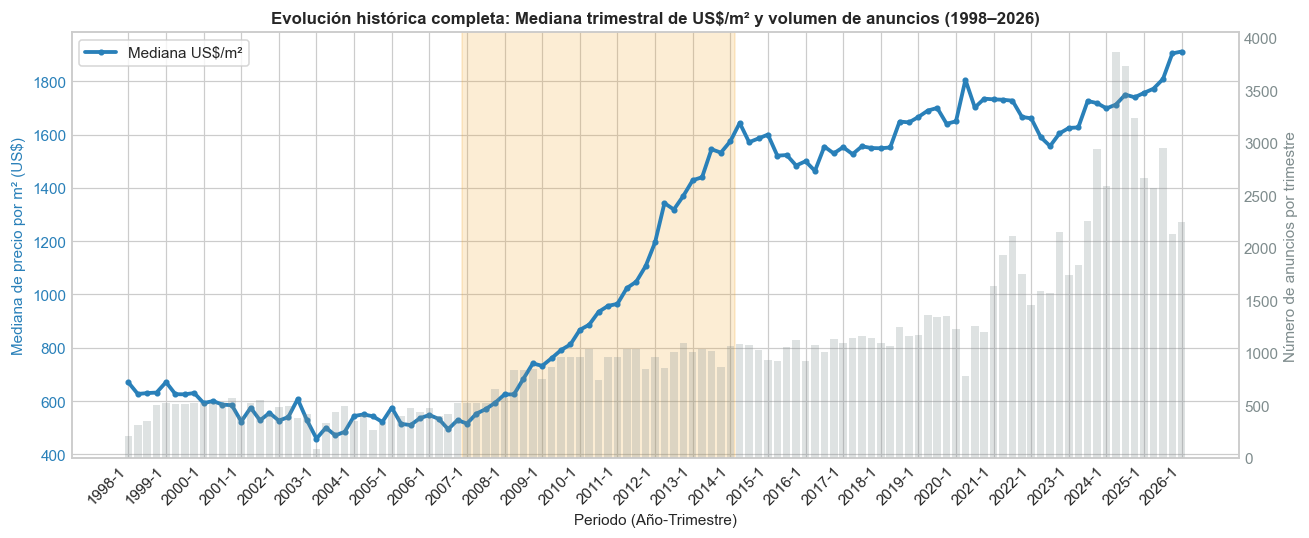
\includegraphics[width=0.88\textwidth]{figures/02a_evolucion_historica_mediana_trimestral_US.png}
    \caption{Evolución histórica de la mediana trimestral de US\$/m$^2$ en Lima Metropolitana (1998--2026).}
    \label{fig:evolucion_historica}
\end{figure}

\noindent \textbf{Interpretación del equipo:}
La triplicación de precios ocurrida entre 2007 y 2014 refleja un cambio estructural exógeno impulsado por el crecimiento del PBI peruano, la masificación del crédito hipotecario bancario y la rápida apreciación del suelo urbano. Por tanto, entrenar un modelo con datos previos a 2014 introduciría un sesgo severo: las valoraciones de 1998--2006 pertenecen a un régimen macroeconómico completamente extinto que distorsionaría las predicciones actuales.

\subsection{Comportamiento del Mercado Contemporáneo}
\noindent \textbf{Lo que muestran los datos:}
Al enfocar el análisis en el segmento contemporáneo (Figura \ref{fig:mercado_contemporaneo}), la mediana trimestral muestra una estabilidad resiliente con variaciones intertrimestrales controladas ($\pm 3\%$), y una dispersión acotada por distrito.

\begin{figure}[H]
    \centering
    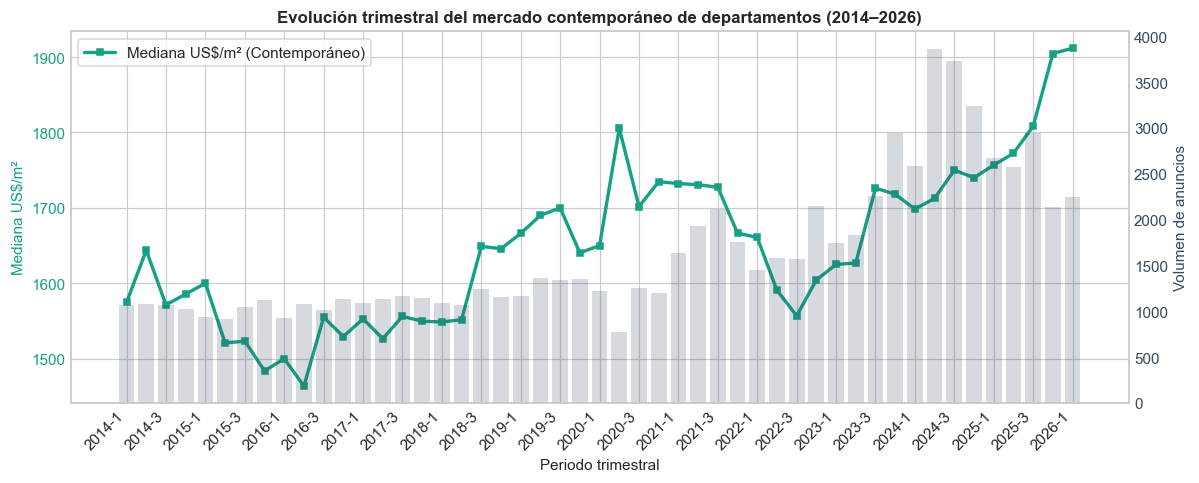
\includegraphics[width=0.85\textwidth]{figures/02b_evolucion_trimetral_mercado_contemporaneo_departamentos.png}
    \caption{Evolución trimestral del mercado contemporáneo de departamentos.}
    \label{fig:mercado_contemporaneo}
\end{figure}

\subsection{Análisis de la Variable Objetivo: Distribución y Transformación}
\noindent \textbf{Lo que muestran los datos:}
La distribución original de la variable \texttt{precio\_usd} exhibe una severa asimetría positiva (\textit{right-skewed}) con una marcada concentración en el rango de US\$ 70,000 a US\$ 200,000 y una cola larga que se extiende hasta US\$ 3,420,000. Al aplicar la transformación logarítmica natural:
\begin{equation}
    y' = \ln(1 + \text{precio\_usd})
\end{equation}
la variable converge hacia una distribución aproximadamente gaussiana y simétrica (Figura \ref{fig:distribucion_precio}).

\begin{figure}[H]
    \centering
    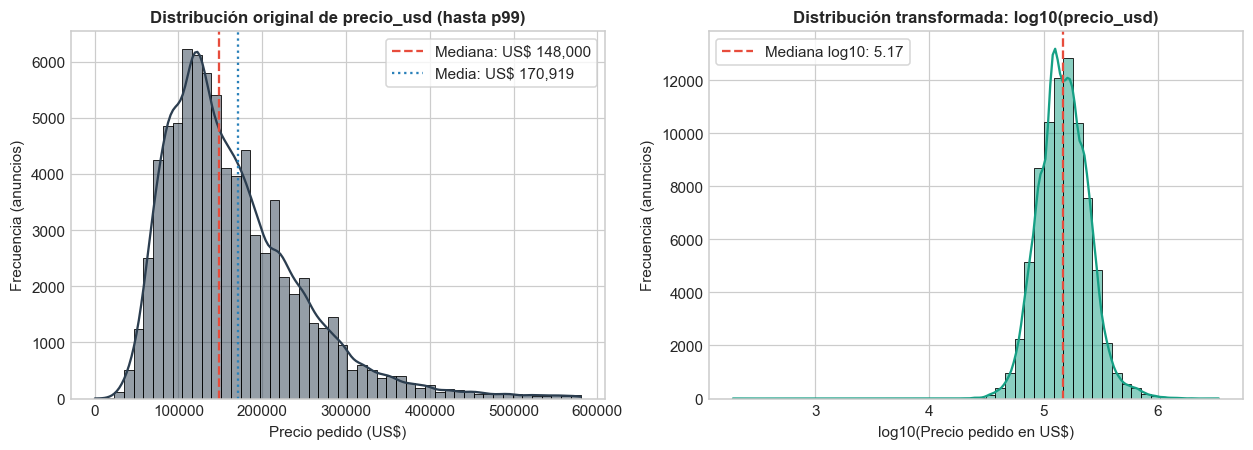
\includegraphics[width=0.88\textwidth]{figures/02c_distribucion_precio_original_transformada.png}
    \caption{Distribución de \texttt{precio\_usd} en escala original (izquierda) y transformada mediante logaritmo (derecha).}
    \label{fig:distribucion_precio}
\end{figure}

\noindent \textbf{Interpretación del equipo:}
Modelar el precio en escala lineal provocaría que los algoritmos (especialmente los basados en pérdida cuadrática como OLS, Ridge o árboles con MSE) concentren casi todo el peso de optimización en minimizar errores absolutos en inmuebles millonarios, descuidando el segmento medio que concentra el 90\% del volumen. La escala logarítmica instruye al modelo a penalizar \textbf{errores porcentuales o relativos}, lo cual es coherente con la negociación inmobiliaria real: errar por US\$ 10,000 en un departamento de US\$ 70,000 es crítico (14.3\%), mientras que en una propiedad de US\$ 1,000,000 representa apenas un 1\%.

\subsection{Relación entre Atributos Físicos y Precio}
\noindent \textbf{Lo que muestran los datos:}
\begin{itemize}[leftmargin=1.5cm]
    \item \textbf{Superficie en m$^2$:} Es el determinante físico principal. En escala logarítmica (Figura \ref{fig:superficie_precio}), la relación entre el área y el precio muestra una correlación lineal positiva muy fuerte ($r \approx 0.82$).
    \item \textbf{Garajes y Habitaciones:} El precio mediano asciende de forma monotónica conforme se incrementa el número de cocheras y dormitorios (Figura \ref{fig:precio_garajes_hab}). La prima por cochera es pronunciada: contar con al menos una cochera incrementa sustancialmente la mediana respecto a unidades sin garaje.
\end{itemize}

\begin{figure}[H]
    \centering
    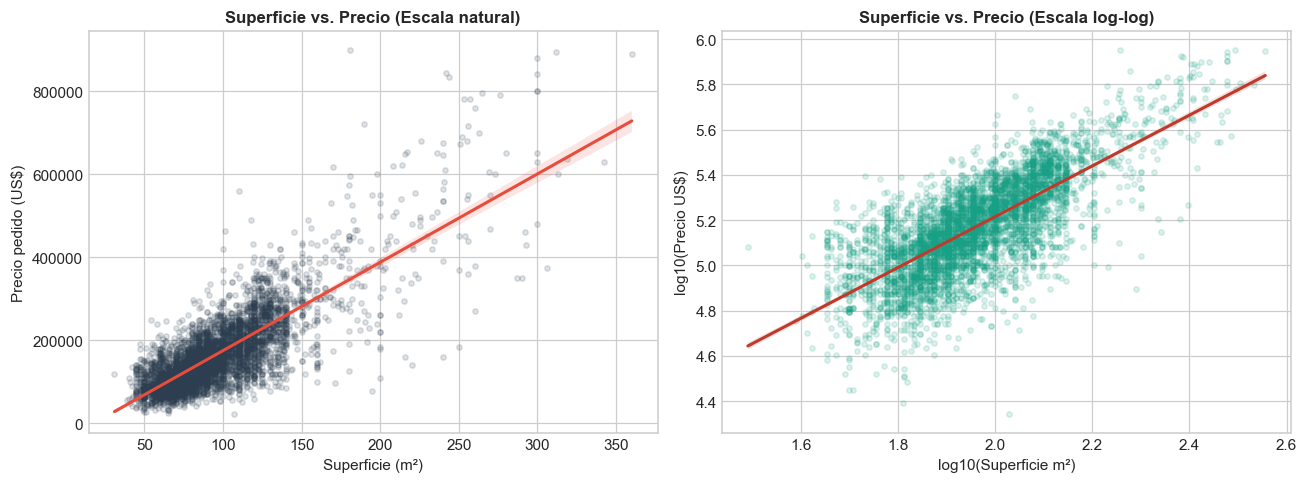
\includegraphics[width=0.85\textwidth]{figures/02e_superficie_vs_precio.png}
    \caption{Dispersión de superficie en m$^2$ vs. precio de oferta en escala logarítmica.}
    \label{fig:superficie_precio}
\end{figure}

\begin{figure}[H]
    \centering
    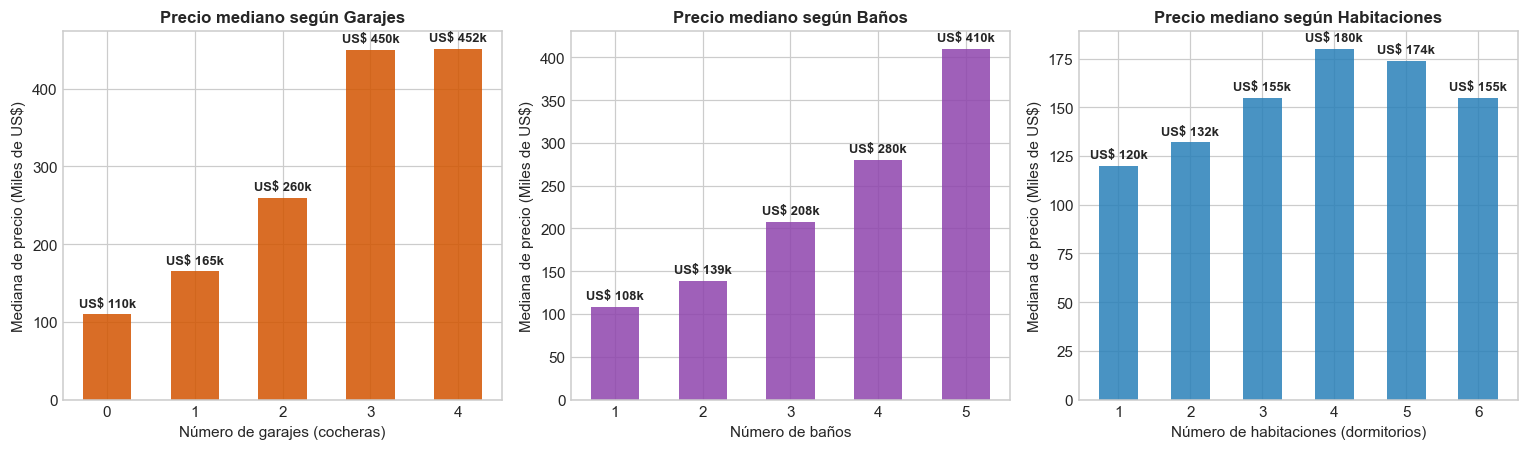
\includegraphics[width=0.85\textwidth]{figures/02f_precio_mediano_garajes_habitaciones.png}
    \caption{Precio mediano según dotación de garajes y habitaciones.}
    \label{fig:precio_garajes_hab}
\end{figure}

\subsection{Heterogeneidad Espacial por Distrito}
\noindent \textbf{Lo que muestran los datos:}
La distribución del precio por metro cuadrado exhibe una segmentación espacial categórica entre conglomerados urbanos de Lima Metropolitana (Figura \ref{fig:precio_distrito}):
\begin{itemize}[leftmargin=1.5cm]
    \item \textbf{Lima Top:} Barranco, San Isidro, Miraflores y San Borja presentan medianas que superan los US\$ 1,900 a US\$ 2,200/m$^2$.
    \item \textbf{Lima Moderna:} Jesús María, Lince, Magdalena, Surquillo y San Miguel oscilan en el rango medio de US\$ 1,500 a US\$ 1,800/m$^2$.
    \item \textbf{Lima Norte / Este / Callao:} Carabayllo, Comas, Los Olivos, Ate y Bellavista registran medianas entre US\$ 800 y US\$ 1,200/m$^2$.
\end{itemize}

\begin{figure}[H]
    \centering
    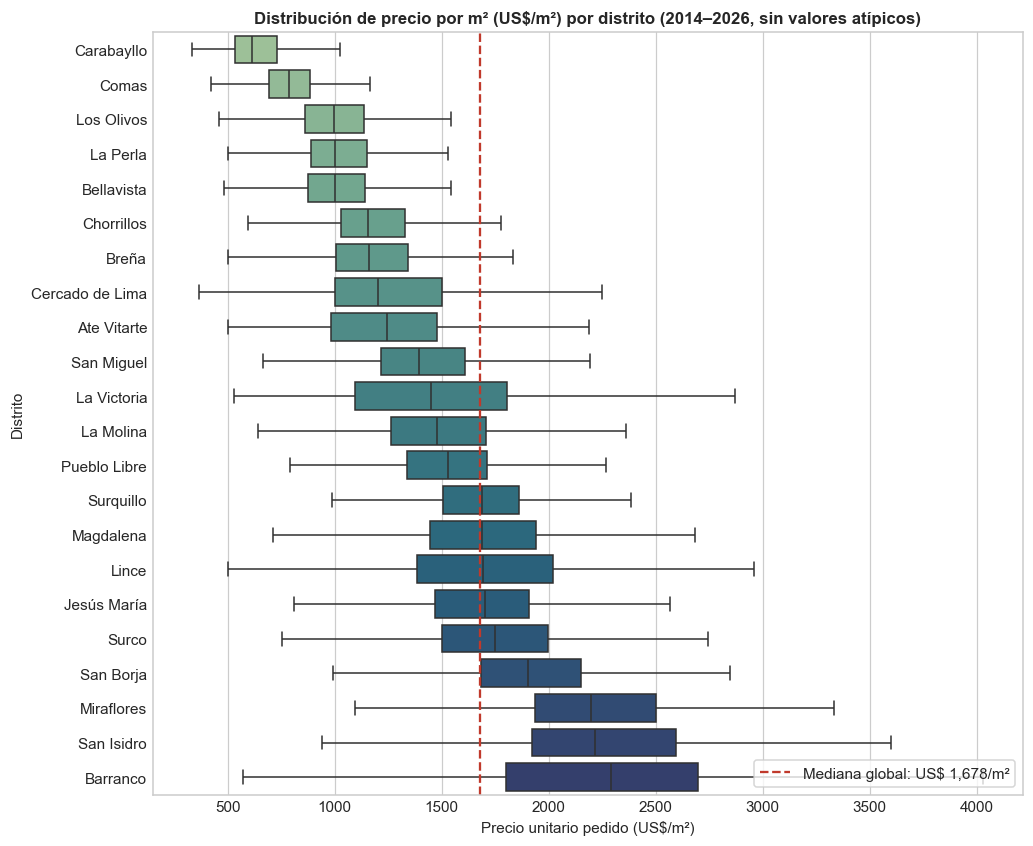
\includegraphics[width=0.92\textwidth]{figures/02g_distribucion_precio_por_distrito.png}
    \caption{Distribución del precio por metro cuadrado segregado por distrito municipal.}
    \label{fig:precio_distrito}
\end{figure}

\noindent \textbf{Interpretación del equipo:}
La variabilidad territorial confirma que la localización es la variable categórica de mayor poder predictivo. Modelos que no capturen efectos fijos distritales o interacciones espaciales cometerán errores masivos de sobreestimación en conos y subestimación en zonas consolidadas.

\subsection{Depreciación Inmobiliaria según Antigüedad}
\noindent \textbf{Lo que muestran los datos:}
El precio por m$^2$ en función de la antigüedad (Figura \ref{fig:depreciacion_antiguedad}) evidencia una curva decreciente con gradiente no lineal: los departamentos de estreno (0 años) y seminuevos (1 a 5 años) capturan una prima premium; entre los 6 y 20 años la curva se estabiliza, mostrando una depreciación marginal decreciente a partir de los 25 años.

\begin{figure}[H]
    \centering
    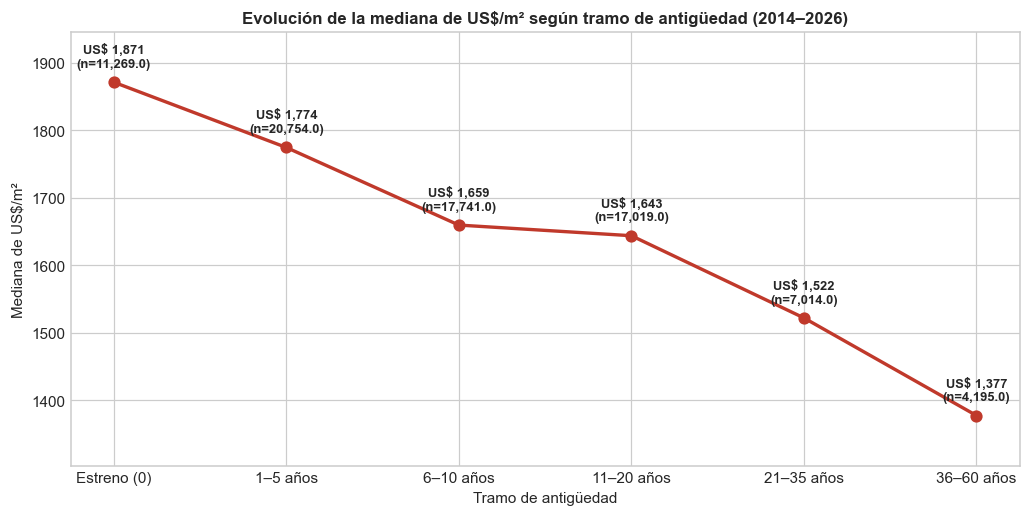
\includegraphics[width=0.85\textwidth]{figures/02h_evolucion_mediana_segun_tramo_antiguedad.png}
    \caption{Evolución de la mediana de precio por m$^2$ según tramos de antigüedad.}
    \label{fig:depreciacion_antiguedad}
\end{figure}

\subsection{Problemas de Calidad que Condicionan Decisiones Posteriores}
Durante el EDA se identificaron dos fallas estructurales de instrumentación en los datos que forzaron decisiones metodológicas fundamentales (Figura \ref{fig:piso_vista_calidad}):
\begin{enumerate}[leftmargin=1.5cm]
    \item \textbf{Discontinuidad en la variable \texttt{piso}:} Hasta 2018, la variable piso se registraba regularmente. Sin embargo, a partir de 2019, más del 98\% de los registros reportan valor 0 o faltante. Si el 0 representara "primer piso", su proporción sería estable en el tiempo; su abrupta concentración al 100\% demuestra que el portal web o el recolector dejó de capturar el dato.
    \item \textbf{Colapso a valor constante en \texttt{vista\_exterior}:} Desde 2022, el 100\% de las observaciones con valor reportado registran exactamente \texttt{1.0} (vista a la calle), perdiendo toda capacidad de discriminación.
\end{enumerate}

\begin{figure}[H]
    \centering
    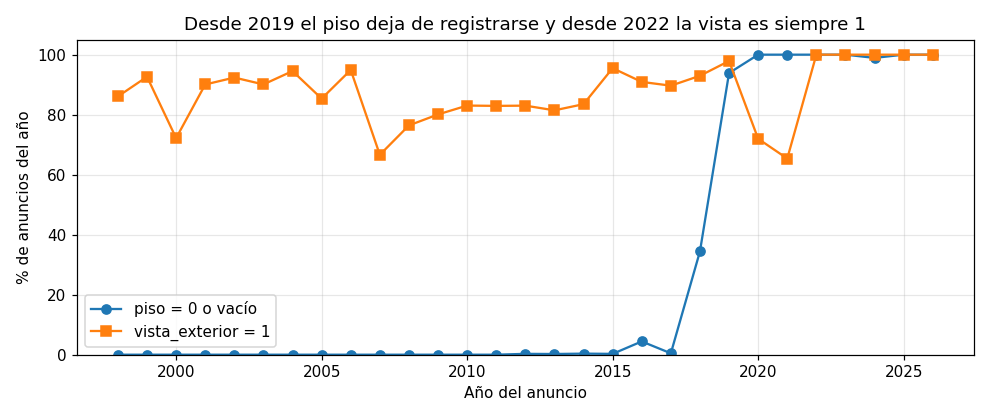
\includegraphics[width=0.85\textwidth]{figures/01_piso_vista_por_anio.png}
    \caption{Porcentaje de anomalías por año en \texttt{piso} (0 o nulo) y \texttt{vista\_exterior} (constante 1).}
    \label{fig:piso_vista_calidad}
\end{figure}

\noindent \textbf{Decisión del equipo:} Descartar formalmente \texttt{piso} y \texttt{vista\_exterior} de la matriz de entrenamiento para evitar alimentar a los modelos con ruido o variables degeneradas.

% ==============================================================================
\section{Calidad y Preparación de Datos}
% ==============================================================================

\subsection{Eliminación de Duplicados}
Se identificaron y eliminaron \textbf{2,730 filas idénticas exactas} presentes en el archivo original del BCRP. Esta deduplicación se aplicó de manera preliminar antes de cualquier división para asegurar que anuncios repetidos por re-publicación de portales no inflaran artificialmente la masa muestral.

\subsection{Normalización de Categorías Inconsistentes}
La columna \texttt{distrito} presentaba originalmente 44 valores textuales únicos debido a discrepancias de digitación, mezcla de mayúsculas y minúsculas (ej. \textit{"SURCO"}, \textit{"surco"}, \textit{"Surco"}), y espacios residuales. Mediante la función \texttt{normalizar\_distritos}, se unificaron las grafías en \textbf{26 distritos canónicos oficiales}, asignando la denominación más frecuente a cada clave normalizada.

\subsection{Corrección de Valores Imposibles (Reglas Lógicas y de Negocio)}
Se implementaron filtros de consistencia lógica para atributos físicos:
\begin{itemize}[leftmargin=1.5cm]
    \item \textbf{Número de baños:} Los baños deben ser enteros o medios baños (visitas). Se verificó que $(2 \times \text{baños}) \pmod 1 == 0$. Cualquier valor que no cumpliera la regla o valores atípicos ($> 9$) fueron convertidos a \texttt{np.nan} para posterior imputación.
    \item \textbf{Antigüedad del edificio:} Se encontraron registros con antigüedad de hasta 1,996 años (anuncios donde se digitó el año de construcción en lugar de los años transcurridos). Toda antigüedad superior a 150 años fue reclasificada como faltante (\texttt{np.nan}).
\end{itemize}

\subsection{Eliminación de Fuga de Datos (\textit{Data Leakage}) y Redundancias}
El Cuadro \ref{tab:fuga_datos} fundamenta la exclusión de cinco variables originales del BCRP.

\begin{table}[H]
\centering
\small
\caption{Justificación técnica del descarte de columnas por fuga o redundancia.}
\label{tab:fuga_datos}
\begin{tabularx}{\textwidth}{lp{4cm}X}
\toprule
\textbf{Columna} & \textbf{Condición Técnica} & \textbf{Justificación de Exclusión} \\
\midrule
\texttt{precio\_soles} & $\text{precio\_usd} \times \text{tipo\_cambio}$ & \textbf{Fuga de datos flagrante.} Es la variable objetivo multiplicada por una constante. Incluirla permitiría al modelo "predecir" el precio con $R^2 = 1.0$ sin aprender nada del inmueble. \\
\texttt{precio\_soles\_2009} & $(\text{precio\_soles} / \text{ipc}) \times 100$ & \textbf{Fuga de datos.} Cálculo aritmético directo sobre el precio objetivo deflactado. \\
\texttt{tipo\_cambio} & Idéntico en el trimestre & \textbf{Redundante.} Se conoce a nivel macroeconómico y está totalmente subsumido por el año y trimestre. \\
\texttt{ipc} & Idéntico en el trimestre & \textbf{Redundante.} Subsumido por la fecha. \\
\texttt{periodo} & Texto (\textit{'2024-1'}) & \textbf{Redundante.} Información descompuesta en \texttt{anio} y \texttt{trimestre}. \\
\bottomrule
\end{tabularx}
\end{table}

\subsection{Filtro de Valores Extremos y Outliers por Distrito}
Se diseñó un estimador especializado (\texttt{FiltroPrecioM2Extremo} / \texttt{FiltroIQRDistrito}) para eliminar publicaciones con precios por metro cuadrado aberrantes (por ejemplo, errores tipográficos donde se anunció US\$ 190 por un departamento completo o US\$ 50,000/m$^2$ por error en la moneda).
\begin{itemize}[leftmargin=1.5cm]
    \item \textbf{Principio anti-fuga:} Los límites del filtro se calculan \textbf{exclusivamente sobre el conjunto de entrenamiento} utilizando la mediana de US\$/m$^2$ por distrito y año:
    \begin{equation}
        \text{Ratio} = \frac{\text{Precio\_USD} / \text{Superficie\_m2}}{\text{Mediana}(\text{US\$/m}^2)_{\text{distrito, anio}}}
    \end{equation}
    \item Se descartan aquellas observaciones cuyo ratio sea menor a 0.25 (menos de la cuarta parte del precio típico zonal) o mayor a 4.0 (más de cuatro veces el valor zonal).
\end{itemize}

% ==============================================================================
\section{Separación de los Datos}
% ==============================================================================

\subsection{Estrategia de Partición Temporal (\textit{Out-of-Time})}
En problemas de tasación y valoración comercial, una partición aleatoria convencional (\textit{K-Fold Cross-Validation} o \textit{train\_test\_split} aleatorio) constituye una violación metodológica grave conocida como \textbf{fuga de datos temporal (\textit{temporal data leakage})}. En un escenario aleatorio, el algoritmo utilizaría información de precios de anuncios contemporáneos o futuros para predecir anuncios pasados, inflando ficticiamente las métricas de precisión.

Por ende, se adoptó una estrategia estricta de \textbf{partición temporal fuera de muestra (\textit{Hold-Out Temporal})}:
\begin{itemize}[leftmargin=1.5cm]
    \item \textbf{Horizonte acotado contemporáneo:} Se seleccionaron los datos del período \textbf{2022-T1 a 2026-T1} ($N = 40,368$ antes de filtro). Este corte garantiza dos requisitos indispensables: estabilidad macroeconómica post-pandemia y la presencia activa de los \textbf{26 distritos metropolitanos}.
    \item \textbf{Conjunto de Entrenamiento (Train):} Años \textbf{2022 y 2023} (8 trimestres). Tras el filtro de extremos ajustado en esta muestra, contiene \textbf{15,158 observaciones} (37.7\% de la muestra filtrada).
    \item \textbf{Conjunto de Evaluación (Test):} Años \textbf{2024 a 2026-T1} (9 trimestres). Tras aplicar los límites aprendidos en Train, contiene \textbf{25,048 observaciones} (62.3\% de la muestra filtrada).
\end{itemize}

\subsection{Medidas Adoptadas para Evitar Data Leakage}
Para blindar el experimento contra cualquier transferencia indebida de información:
\begin{enumerate}[leftmargin=1.5cm]
    \item La imputación de valores faltantes (medianas de baños, garajes y antigüedad) se calculó exclusivamente sobre el conjunto Train.
    \item Los parámetros de centrado y escala del \texttt{RobustScaler} se ajustaron (\texttt{fit}) únicamente con Train y se aplicaron (\texttt{transform}) a Test.
    \item El codificador \texttt{OneHotEncoder} para distritos se ajustó exclusivamente con Train, configurando \texttt{handle\_unknown='ignore'} para asegurar que si Test presentara una categoría inédita, se codifique como ceros sin generar errores.
    \item El filtro de outliers de precio/m$^2$ aprendió sus cuantiles y medianas en Train y se proyectó sobre Test sin reajustarse.
\end{enumerate}

% ==============================================================================
\section{Flujo Reproducible de Preprocesamiento}
% ==============================================================================

Para garantizar la reproducibilidad y permitir un despliegue directo a producción en una interfaz web, todo el flujo de transformación de variables de entrada se encapsuló en un \texttt{ColumnTransformer} nativo de Scikit-Learn (Listado \ref{lst:pipeline}).

\begin{lstlisting}[language=Python, caption={Definición del Pipeline y ColumnTransformer de preprocesamiento.}, label={lst:pipeline}]
from sklearn.pipeline import Pipeline
from sklearn.compose import ColumnTransformer, TransformedTargetRegressor
from sklearn.impute import SimpleImputer
from sklearn.preprocessing import RobustScaler, OneHotEncoder
import numpy as np

# 1. Definicion de atributos por tipologia
cols_num = ['superficie_m2', 'habitaciones', 'banos', 'garajes', 'antiguedad_anios']
cols_cat = ['distrito']

# 2. Pipeline para caracteristicas numericas
num_pipeline = Pipeline([
    ('imputer', SimpleImputer(strategy='median')),
    ('scaler', RobustScaler())
])

# 3. Pipeline para caracteristicas categoricas
cat_pipeline = Pipeline([
    ('encoder', OneHotEncoder(handle_unknown='ignore', sparse_output=False))
])

# 4. Ensamble en ColumnTransformer integrado
preprocesador = ColumnTransformer([
    ('num', num_pipeline, cols_num),
    ('cat', cat_pipeline, cols_cat)
], remainder='drop')
\end{lstlisting}

\noindent\textbf{Justificación de los transformadores:}

\begin{itemize}[leftmargin=1.5cm]
    \item \texttt{SimpleImputer(strategy='median')}: 
    Robusto ante la asimetría de variables discretas como garajes o antigüedad.

    \item \texttt{RobustScaler()}: 
    Escala restando la mediana y dividiendo por el rango intercuartílico (IQR), 
    previniendo que valores legítimos en la cola superior 
    (ej. penthouses de 500 m$^2$) colapsen los pesos de los modelos lineales.

    \item \texttt{TransformedTargetRegressor}: 
    Envuelve a todo el estimador para garantizar que el entrenamiento se realice 
    sobre $\ln(1+y)$ y las predicciones finales retornen automáticamente 
    en dólares corrientes originales.
\end{itemize}

% ==============================================================================
\section{Baselines de Referencia}
% ==============================================================================

Para responder con rigor si los modelos de Machine Learning aportan valor predictivo real, se establecieron tres modelos base de referencia:
\begin{enumerate}[leftmargin=1.5cm]
    \item \textbf{DummyRegressor (Media):} Predice de forma constante la media global de \texttt{precio\_usd} observada en el entrenamiento (US\$ 144,320). Representa una solución trivial na\"ive.
    \item \textbf{DummyRegressor (Mediana):} Predice de forma constante la mediana global de entrenamiento (US\$ 125,000).
    \item \textbf{Regla de Mercado (\texttt{ReglaMercadoM2}):} Estima el precio aplicando la heurística clásica de tasación:
    \begin{equation}
        \widehat{y}_i = \text{Mediana}\left(\frac{\text{precio\_usd}}{\text{superficie\_m2}}\right)_{\text{distrito}, \text{Train}} \times \text{superficie\_m2}_i
    \end{equation}
    Esta regla fue encapsulada como un estimador formal de Scikit-Learn (\texttt{BaseEstimator, RegressorMixin}) para integrarse de manera idéntica al protocolo de evaluación.
\end{enumerate}

% ==============================================================================
\section{Modelos Preliminares}
% ==============================================================================

Se seleccionaron cuatro familias de algoritmos supervisados, cubriendo tanto modelos paramétricos lineales regularizados como ensambles no lineales basados en árboles:
\begin{enumerate}[leftmargin=1.5cm]
    \item \textbf{Ridge Regressor (Regresión Lineal con Penalización $L_2$):}
    \begin{equation}
        \min_{\mathbf{w}} \left\{ \|\mathbf{y}_{log} - \mathbf{X}\mathbf{w}\|_2^2 + \alpha \|\mathbf{w}\|_2^2 \right\}
    \end{equation}
    Configurado con $\alpha = 1.0$. Permite evaluar la capacidad explicativa lineal sobre el espacio logarítmico manteniendo estabilidad ante la correlación entre ambientes físicos.
    \item \textbf{ElasticNet (Penalización combinada $L_1 + L_2$):}
    Configurado con $\alpha = 0.1$ y ratio de mezcla $L_1 = 0.5$. Busca inducir dispersión en los coeficientes preservando la selección de variables en bloque.
    \item \textbf{Random Forest Regressor:} Ensamble de \textit{bagging} con 100 árboles de decisión y profundidad máxima de 15 niveles (\texttt{max\_depth=15}). Diseñado para capturar no linealidades e interacciones de orden superior (por ejemplo, que una cochera tenga un valor marginal muy superior en San Isidro que en Carabayllo).
    \item \textbf{CatBoost Regressor:} Algoritmo de \textit{Gradient Boosting} especializado en árboles simétricos (\textit{oblivious trees}). Configurado con 200 iteraciones, profundidad 8 y tasa de aprendizaje adaptativa. Es altamente resistente al sobreajuste y eficiente en datos tabulares heterogéneos.
\end{enumerate}

% ==============================================================================
\section{Evaluación Preliminar y Comparación de Modelos}
% ==============================================================================

\subsection{Selección y Justificación de Métricas}
En valoración inmobiliaria, evaluar con una única métrica es insuficiente. Se seleccionaron cinco métricas complementarias (Cuadro \ref{tab:metricas_desc}):
\begin{itemize}[leftmargin=1.5cm]
    \item \textbf{MAE (Error Absoluto Medio):} Magnitud promedio del error en dólares: $\frac{1}{N}\sum |y_i - \widehat{y}_i|$.
    \item \textbf{RMSE (Raíz del Error Cuadrático Medio):} Penaliza con severidad los errores catastróficos en inmuebles costosos.
    \item \textbf{Error \% Mediano (MedAPE):} Métrica clave del negocio. Al ser la mediana de los errores relativos $|\frac{y_i - \widehat{y}_i}{y_i}|$, no se ve distorsionada por unos pocos anuncios atípicos y refleja el error típico de una tasación.
    \item \textbf{MAPE (Error Porcentual Absoluto Medio):} Promedio de los errores relativos.
    \item \textbf{\% Anuncios con error $\le$ 10\%:} Proporción de propiedades tasadas dentro del margen de negociación estándar de mercado.
\end{itemize}

\begin{table}[H]
\centering
\small
\caption{Resultados comparativos en el conjunto de prueba temporal (2024--2026, $N = 25,048$).}
\label{tab:resultados_comparativos}
\begin{tabularx}{\textwidth}{lccccc}
\toprule
\textbf{Modelo / Estimador} & \textbf{MAE} & \textbf{RMSE} & \textbf{Error \% Mediano} & \textbf{MAPE} & \textbf{Error $\le$ 10\%} \\
\midrule
Dummy (Media) & 53,386 & 69,653 & 28.6\% & 36.9\% & 17.2\% \\
Dummy (Mediana) & 54,908 & 73,539 & 28.9\% & 34.7\% & 18.6\% \\
\textbf{Regla de mercado} & \textbf{28,597} & \textbf{38,350} & \textbf{14.9\%} & \textbf{18.4\%} & \textbf{34.5\%} \\
\midrule
Ridge Regressor & 24,385 & 33,847 & 12.3\% & 15.1\% & 41.3\% \\
ElasticNet & 38,028 & 52,053 & 19.4\% & 23.9\% & 26.3\% \\
Random Forest Regressor & 23,942 & 33,781 & 11.8\% & 14.9\% & 43.5\% \\
\textbf{CatBoost Regressor} & \textbf{23,000} & \textbf{32,685} & \textbf{11.3\%} & \textbf{14.2\%} & \textbf{45.3\%} \\
\bottomrule
\end{tabularx}
\end{table}

\subsection{Interpretación Técnica de Resultados}
La evidencia empírica condensada en el Cuadro \ref{tab:resultados_comparativos} arroja conclusiones técnicas fundamentales:
\begin{enumerate}[leftmargin=1.5cm]
    \item \textbf{CatBoost es el modelo ganador indiscutible:} Logra el menor error porcentual mediano (\textbf{11.3\%}), superando por \textbf{3.6 puntos porcentuales} a la regla de mercado (14.9\%). Asimismo, incrementa la proporción de anuncios tasados con alta precisión comercial ($\le 10\%$) del 34.5\% al \textbf{45.3\%}.
    \item \textbf{Reducción del Riesgo Financiero:} El RMSE se redujo de US\$ 38,350 a \textbf{US\$ 32,685} (una disminución de más de US\$ 5,600), demostrando que CatBoost controla eficazmente desviaciones en propiedades de alto valor.
    \item \textbf{Competitividad de Ridge vs. Fracaso de ElasticNet:} Ridge obtuvo un sobresaliente 12.3\% de MedAPE, confirmando que la combinación de escala logarítmica y \texttt{RobustScaler} linealiza con éxito gran parte del fenómeno. Por el contrario, ElasticNet (19.4\%) no logró batir a la regla de mercado debido a que su penalización $L_1$ por defecto comprimió en exceso coeficientes distritales cruciales.
\end{enumerate}

\subsection{Diagnóstico de Residuales del Modelo CatBoost}
Al analizar el gráfico de dispersión de valores reales frente a predichos (Figura \ref{fig:catboost_residuales}), se constatan dos patrones diagnósticos esenciales:

\begin{figure}[H]
    \centering
    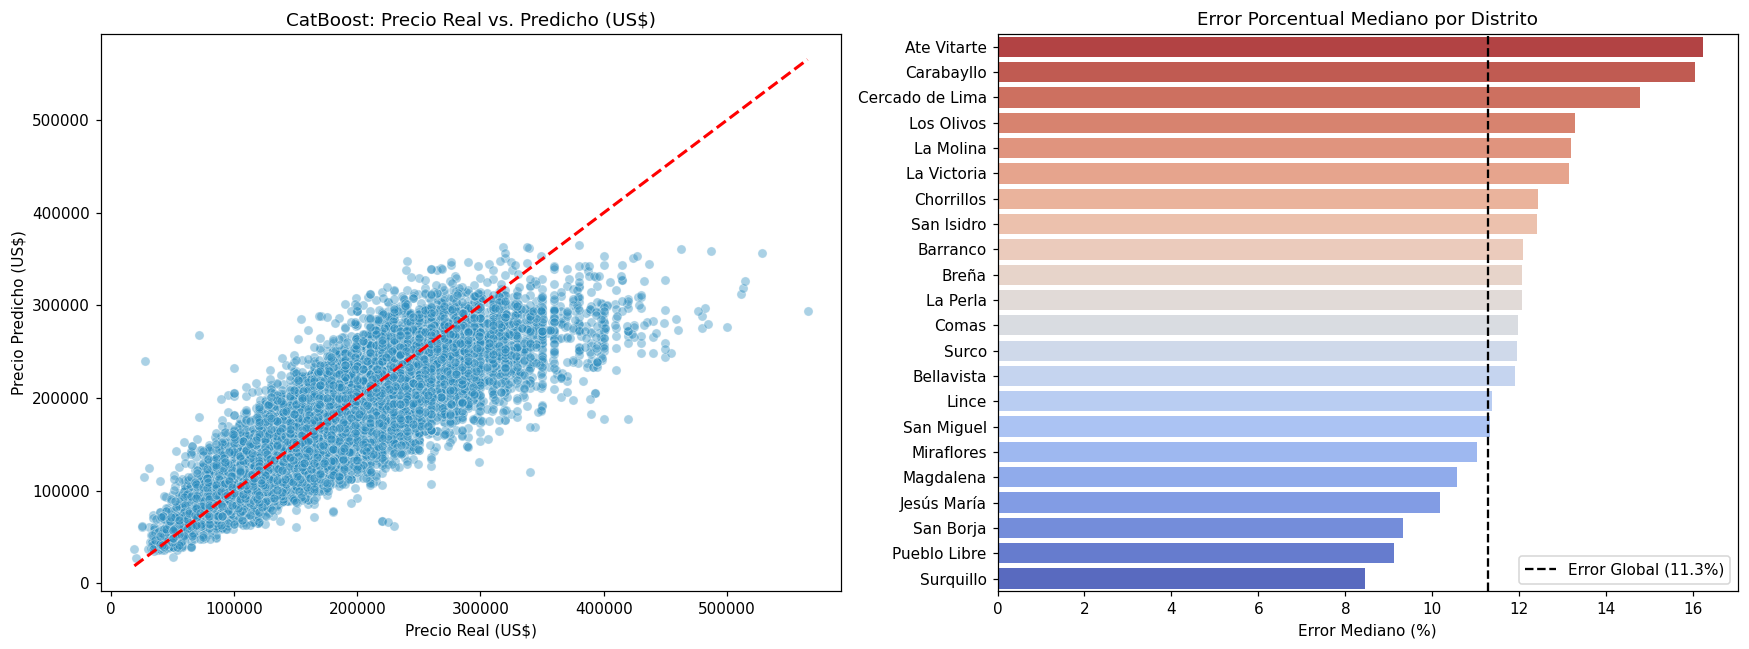
\includegraphics[width=0.88\textwidth]{figures/03_catboost_precio_real_vs_predicho.png}
    \caption{Diagnóstico de residuales del modelo CatBoost: Precio real vs. precio predicho en escala original (US\$).}
    \label{fig:catboost_residuales}
\end{figure}

\begin{enumerate}[leftmargin=1.5cm]
    \item \textbf{Alta fidelidad en el segmento estándar:} Entre US\$ 50,000 y US\$ 250,000, los puntos se alinean con extraordinaria densidad a lo largo de la diagonal ideal ($y = \widehat{y}$).
    \item \textbf{Techo predictivo en el segmento de ultralujo ($> \text{US\$} 350,000$):} El modelo tiende a aplanar la curva, subestimando sistemáticamente los departamentos de lujo extremo. La causa raíz radica en la ausencia de atributos cualitativos en la base del BCRP (acabados de lujo, diseño arquitectónico, vista directa al mar o campos de golf).
    \item \textbf{Disparidad periférica:} En distritos con escasa masa crítica en entrenamiento (ej. Carabayllo), los errores relativos crecen sustancialmente producto del desbalance muestral geográfico histórico.
\end{enumerate}

% ==============================================================================
\section{Estado del Proyecto y Plan hacia el TF1}
% ==============================================================================

\subsection{Principales Hallazgos hasta el Momento}
\begin{itemize}[leftmargin=1.5cm]
    \item La regla empírica del mercado limeño (US\$/m$^2$ $\times$ área) comete un error porcentual mediano del 14.9\% en el período contemporáneo.
    \item El modelado con Machine Learning supervisado (especialmente CatBoost y Random Forest) sobre la variable objetivo transformada logarítmicamente reduce el error mediano a un competitivo \textbf{11.3\%}, demostrando viabilidad y utilidad comercial práctica.
    \item El momento del mercado y la localización distrital dominan la varianza, pero la dotación de cocheras y antigüedad explican los diferenciales finos entre pares comparables.
\end{itemize}
san 
\subsection{Problemas No Resueltos y Limitaciones Identificadas}
\begin{enumerate}[leftmargin=1.5cm]
    \item \textbf{Subestimación en ultralujo:} El modelo no cuenta con descriptores para capturar el valor intangible en propiedades que superan los US\$ 400,000.
    \item \textbf{Sesgo geográfico en conos:} Distritos periféricos recientemente incorporados sufren tasas de error superiores al 30\% debido a la escasez de datos históricos relativos y posibles errores de tipificación de inmuebles en los anuncios.
    \item \textbf{Duplicados residuales sutiles:} Se identificaron 4 observaciones residuales con idénticos atributos físicos y distritales pero ligeras discrepancias temporales pendientes de auditoría profunda.
\end{enumerate}

\subsection{Mejoras Metodológicas Planificadas para el TF1}
Hacia la entrega del Trabajo Final (TF1), se ejecutarán las siguientes mejoras técnicas:
\begin{enumerate}[leftmargin=1.5cm]
    \item \textbf{Optimización Bayesiana de Hiperparámetros con Optuna:} Afinar iteraciones, profundidad, tasa de aprendizaje y regularización $L_2$ de CatBoost y LightGBM bajo un esquema de validación cruzada temporal (\texttt{TimeSeriesSplit}).
    \item \textbf{Ingeniería de Características Espaciales:} Agrupar los distritos en macrozonas económicas homogéneas (Lima Top, Lima Moderna, Lima Centro, Lima Este, Lima Norte, Lima Sur, Callao) e interactuar variables (ej. ratio baños por dormitorio, m$^2$ por garaje).
    \item \textbf{Interpretabilidad Global y Local con SHAP (\textit{SHapley Additive exPlanations}):} Implementar \texttt{TreeSHAP} para generar gráficos de importancia de variables (\textit{summary plots}) y explicaciones locales tipo \textit{waterfall} que desglosen exactamente cuántos dólares aporta cada atributo a una tasación individual.
    \item \textbf{Estratificación y Balanceo Espacial:} Evaluar ponderaciones muestrales inversas a la frecuencia distrital (\textit{sample weighting}) para mitigar el sesgo hacia distritos de altos ingresos.
    \item \textbf{Despliegue de Aplicación Interactiva en Streamlit:} Construir una plataforma web donde un usuario ingrese el distrito, metraje, ambientes, cocheras y antigüedad, recibiendo la tasación instantánea en dólares, un intervalo de confianza y la explicación visual de SHAP.
\end{enumerate}

\subsection{Cronograma de Actividades hacia el TF1}
El Cuadro \ref{tab:cronograma} sintetiza la planificación y distribución de responsabilidades del equipo de trabajo.

\begin{table}[H]
\centering
\small
\caption{Plan de trabajo y cronograma de actividades hacia el Trabajo Final (TF1).}
\label{tab:cronograma}
\begin{tabularx}{\textwidth}{lp{6.5cm}ccX}
\toprule
\textbf{Semana} & \textbf{Actividad / Entregable} & \textbf{Responsable} & \textbf{Herramientas} \\
\midrule
Semana 9 & Auditoría fina de duplicados residuales e ingeniería de variables compuestas (macrozonas) & Gabriel & pandas, scikit-learn \\
Semana 10 & Configuración de validación cruzada temporal (\texttt{TimeSeriesSplit}) y optimización con Optuna & José & Optuna, CatBoost \\
Semana 11 & Análisis de interpretabilidad con SHAP (valores Shapley globales y locales) & Marcos & SHAP, Matplotlib \\
Semana 12 & Desarrollo de la interfaz interactiva de tasación en Streamlit & Yair & Streamlit, Python \\
Semana 13 & Pruebas de integración, empaquetado del pipeline final y redacción del informe TF1 & Todo el equipo & Git, LaTeX \\
Semana 14 & Ensayos de presentación y consolidación del repositorio final & Todo el equipo & GitHub, Overleaf \\
\bottomrule
\end{tabularx}
\end{table}

% ==============================================================================
\section{Referencias}
% ==============================================================================
\begin{enumerate}[leftmargin=1.5cm]
    \item Banco Central de Reserva del Perú (BCRP). (2018). \textit{Indicadores del mercado inmobiliario y precios hedónicos en Lima Metropolitana}. Documento de Trabajo N° 006-2018.
    \item Banco Central de Reserva del Perú (BCRP). (2025). \textit{Evolución reciente de los precios de venta y alquiler de departamentos en Lima}. Nota de Estudios N° 65-2025.
    \item Prokhorenkova, L., Gusev, G., Vorobev, A., Dorogush, A. V., \& Gulin, A. (2018). \textit{CatBoost: unbiased boosting with categorical features}. Advances in Neural Information Processing Systems (NeurIPS), 31.
    \item Lundberg, S. M., \& Lee, S. I. (2017). \textit{A unified approach to interpreting model predictions}. Advances in Neural Information Processing Systems (NeurIPS), 30.
    \item Pedregosa, F., et al. (2011). \textit{Scikit-learn: Machine Learning in Python}. Journal of Machine Learning Research, 12, 2825--2830.
\end{enumerate}

\end{document}
